\documentclass[../main.tex]{subfile}
\begin{document}
\section{Lecture 1 - proposition and logic}
\subsection{Introduction to Propositions}
\begin{definition}
	proposition is either true or false
\end{definition}
\begin{remark}
	contradiction is not a proposition	
\end{remark}


\begin{definition}[Conditional statement]
	$p \to q$, p is the \vocab{hypothesis}, and q is the \vocab{conclusion}. If the statement is true, then p is the \vocab{necessary condition} and q is the \vocab{sufficient condition}
\end{definition} 

\subsection{Compound propositions}
\begin{enumerate}
	\item converse: $p \to \neg q$
	\item contrapositive: $\neg q \to \neg p$
	\item inverse: $\neg p \to \neg q$
\end{enumerate}

\begin{definition}[Biconditional statement]
$p \iff q$ means p if and only if q, also means p $\equiv$ q	
\end{definition}

\begin{figure}[h!]
\centering
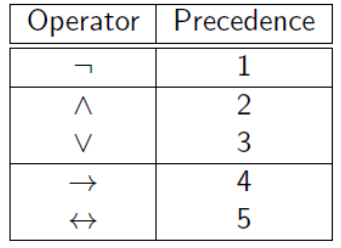
\includegraphics[width=0.5\textwidth]{1-precedence_table.png}
\caption{precedence table}
\label{fig:}
\end{figure}
\subsection{Propositional Equivalence}
\begin{definition}[tautology] A compound proposition that is always \bful{true}, no matter what the truth values of the propositional variables that occur in it.
\end{definition}
	\begin{definition}[contradiction] A compound proposition that is always \bful{false}
	\end{definition}
	\begin{definition}[contingency]A compound proposition that is neither a tautology nor a contradiction
	
\end{definition}	
\begin{figure}[h!]
\centering
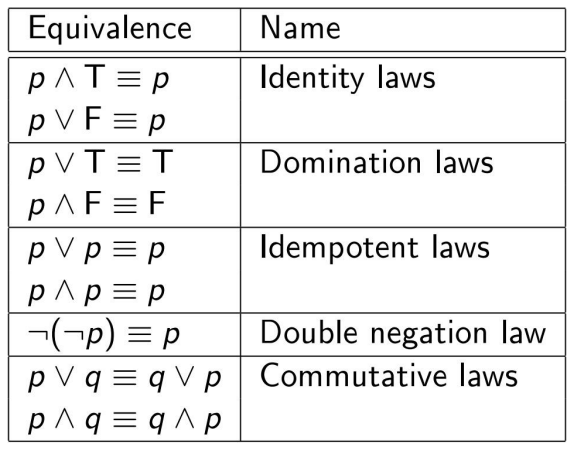
\includegraphics[width=0.5\textwidth]{1-propositional_equivalences.png}
\caption{propositional equivalences}
% \label{fig:}
\end{figure}
\begin{figure}[h!]
\centering
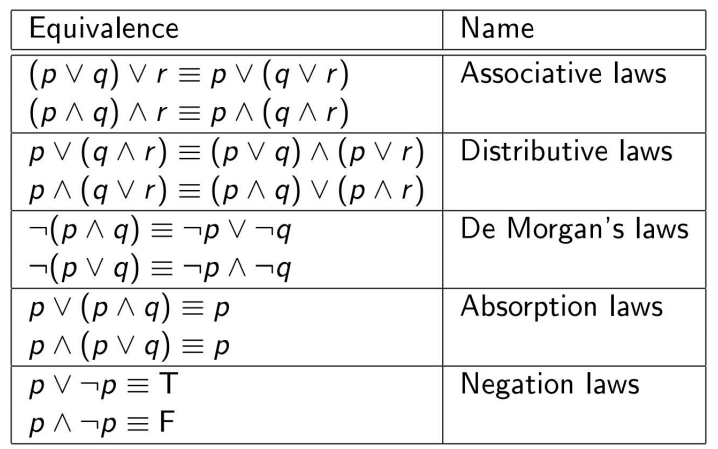
\includegraphics[width=0.5\textwidth]{1-propositional_equivalences_2.png}
\caption{propositional equivalences}
% \label{fig:}
\end{figure}
\begin{figure}[h!]
\centering
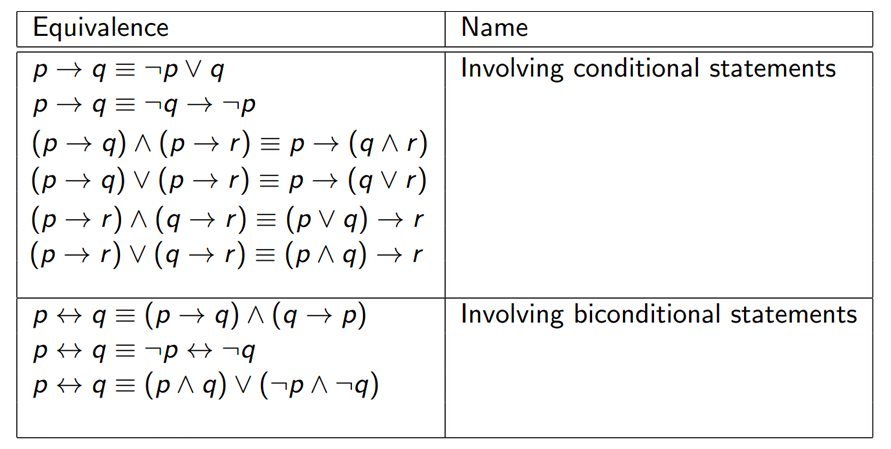
\includegraphics[width=0.8\textwidth]{1-propositional_equivalences_3.png}
\caption{propositional equivalences}
% \label{fig:}
\end{figure}
\clearpage
\end{document}


